% This is samplepaper.tex, a sample chapter demonstrating the
% LLNCS macro package for Springer Computer Science proceedings;
% Version 2.20 of 2017/10/04
%
\documentclass[runningheads]{llncs}
%
\usepackage{graphicx}
% Used for displaying a sample figure. If possible, figure files should
% be included in EPS format.
%
% If you use the hyperref package, please uncomment the following line
% to display URLs in blue roman font according to Springer's eBook style:
% \renewcommand\UrlFont{\color{blue}\rmfamily}
% For correct quotation marks (command \enquote)
\usepackage{csquotes}

\begin{document}
%
\title{Interpretable Machine Learning -- A Brief History, State-Of-The-Art and Challenges\thanks{This project is funded by the Bavarian State Ministry of Science and the Arts and coordinated by the Bavarian Research Institute for Digital Transformation (bidt) and supported by the German Federal Ministry of Education and Research (BMBF) under Grant No. 01IS18036A.
The authors of this work take full responsibilities for its content.
}}
%
\titlerunning{IML - History, Methods, Challenges}
% If the paper title is too long for the running head, you can set
% an abbreviated paper title here
%
\author{Christoph Molnar\inst{1}\orcidID{0000-0003-2331-868X}}
%\and
%Second Author\inst{2,3}\orcidID{1111-2222-3333-4444} \and
%Third Author\inst{3}\orcidID{2222--3333-4444-5555}}
%
\authorrunning{Molnar}
% First names are abbreviated in the running head.
% If there are more than two authors, 'et al.' is used.
%
\institute{LMU Munich, Ludwigstr. 33, 80539 Munich, Germany
\email{christoph.molnar@gmail.com}\\
\url{https://www.slds.stat.uni-muenchen.de/people/molnar/}}
%
\maketitle              % typeset the header of the contribution
%
\begin{abstract}
  I present a very short history of the field of interpretable machine learning (IML), give an overview of popular interpretation methods and discuss challenges when interpreting machine learning models.
  This view might be a bit biased through the eyes of a statistician.

\keywords{Interpretable Machine Learning \and Explainable AI}
\end{abstract}
%
%
Interpretability is often a deciding factor when machine learning (ML) is used in a product, a decision process or in research.
With interpretable machine learning (IML) \footnote{We will be using Interpretable Machine Learning and Explainable AI exchangably} the user can find out problems of the ML model, extract insights and justify decisions.
This short paper views IML through a methodological viewpoint, with an emphasis on \textbf{what can we, mathematically and algorithmically, derive from an ML model} and less on the human part.
%I want to give three very common use cases:
%\paragraph{For science:} In applied sciences, data is often modeled with ML nowadays, where before statistical modeling approach would have been used.
%The goal of science is not only to predict the world well, but also to generate further insights.
%Examples are species distribution models in ecology which aim to explain why certain species can be found on certain areas based on e.g. the local climate.
%Here, interpretability of the prediction model is needed to understand why a species, e.g., has a high probability to occur in a specific reason.

\paragraph{A Very Short History of IML.}
A lot of IML research just happened in the last five years.
But learning interpretable models from data has a much longer tradition.
Linear regression models have been used back in 1800 by Gauss, Legendre and Quetelet \cite{stigler1986history,legendre1805nouvelles,gauss1809theoria,quetelet1827recherches}.
Rule-based machine learning (e.g., decision rules and trees) has been an active research areas since the 1980s \cite{furnkranz2012foundations} with some roots reaching back into the 1960s \cite{hajek1966guha}.
Both research on linear regression models and its extensions and rule-based ML remain important and busy research areas to this day and are even blending together (e.g. model-based trees \cite{zeileis2008model} or RuleFit \cite{friedman2008predictive}).
Machine learning research in general also started around that time, e.g., support vector machines in 1974 \cite{vapnik1974theory}, early important work on neural networks in the 1960s and boosting in 1990 \cite{schapire1990strength}.
Interpretability has always been a companion to ML.
A good example for this is the random forest, which I also see as an IML milestone for making ML practical.
Random forests, a black box machine learning model that often works well without tuning, came with a built-in feature importance measure, which contributed to the success.
The evidence that interpretability was success factor are the many citations (>60000 citation on Google Scholar as of September 2020) of the original paper \cite{breiman2001random}, but also of papers improving the importance measure (\cite{strobl2008conditional,strobl2007bias,hapfelmeier2014new,ishwaran2007variable}).
In the 2010s came the deep learning hype, after a deep neural network won the ImageNet challenge.
A few years after that, the IML field really took off (around 2015), judging by frequency of the search terms "Interpretable Machine Learning" and "Explainable AI" on Google (Figure \ref{fig:count} right)and papers published with these terms (Figure \ref{fig:count} left).
\begin{figure}
  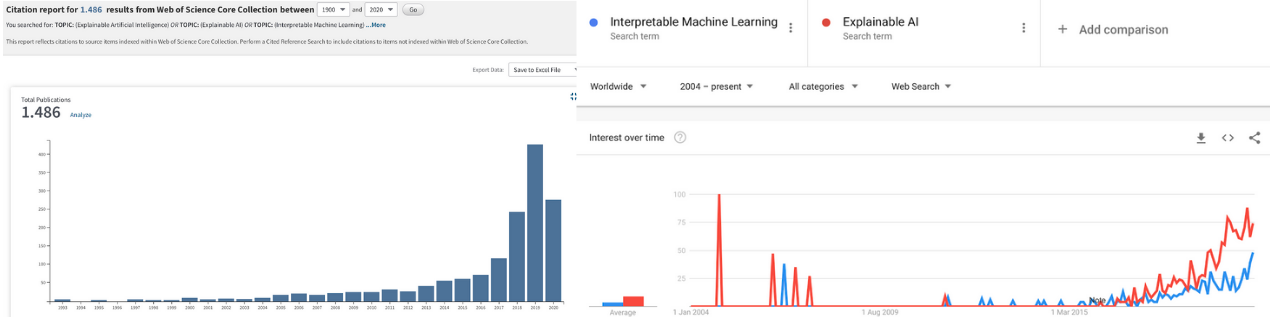
\includegraphics[width=\textwidth]{citation-search.png}
  \caption{Left, Right}
  \label{fig:count}
\end{figure}
Since then, many approaches have been introduced to the field, many of them model-agnostic explanation methods, i.e., working for different types of ML models, but also model-specific explanation methods to interpret, e.g., deep neural networks and tree ensembles.
Rule-based ML and statistical regression models continue to be developed.
%Could it be that only the terms have changed, but the field has always been there and the same?
%I would still argue that the field has reached a new form, as evidenced by new keywords "Interpretable Machine Learning" and "Explainable Artificial Intelligence", but also by bringing in new ideas from other fields, pulling many unconnected research fields together and an additional focus on model-agnostic ML interpretation methods.


\paragraph{Today} IML reached a first state of usability.
Some methods have been established with a better understanding of weaknesses and strengths.
There is a lot of open source software that implement various techniques (\cite{iml,biecek2018dalex,pedregosa2011scikit,klaise2020alibi,nori2019interpretml}, ...) and also big tech companies offer software \cite{exler2019if,arya2020ai,hall2017machine}.
These software tools gives ML practitioners the means to interpret their models.
Regulation such as GDPR has spurred a discussion around further needs of interpretability.
Many startup are now focused on interpretable ML.


\section*{IML Methods}

In this section we broadly cover some popular IML methods.
%Often a distinction is made between model-specific and model-agnostic explanation methods.
%An interpretation method is model-specific if it only works for a specific ML model, it is model-agnostic if it can be applied to any model.
We distinguish IML methods between component and sensitivity analysis\footnote{Not to be confused with the research field of sensitivity analysis, which studies the uncertainty of outputs in mathematical models and systems. But there are methodological overlaps (e.g., Shapley values)}.
An IML method that works by component analysis assigns meaning to \textit{(learned) model parameters and structures} while sensitivity analysis \textit{probes the model with artificial data points and describes its behavior}.\footnote{Some surveys \cite{vilone2020explainable,guidotti2018survey} divide methods into \textit{ante-hoc (alternatively: transparent design, white box models)} and \textit{post-hoc} IML method, depending on whether interpretability is considered at model design and training or after training, leaving the (black-box) model unchanged. Another category divides model-agnostic and model-specific. Component vs. sensitivity analysis is, in our opinion, another interesting view and why only repeat what others already have said?}
The idea of component analysis is closely related to decomposability:
You can only analyse components of a model that can be decomposed into individual components that we can interpret individually.
Component analysis does not necessarily require that the user understands the model in its entirety (simulatability).
The introspection is always model-specific, e.g., a linear regression model can be interpreted by analyzing its coefficients, while a decision tree can be interpreted by visualizing the learned decision structure.
Sensitivity analysis is mostly model-agnostic and works by manipulating input data and analyzing ML model  predictions.
Some IML sensitivity analysis methods rely on model-specific knowledge such as gradients of neural networks. An example are the various heatmap-like explanation for CNNs for image classification \cite{sundararajan2017axiomatic,lundberg2017unified,montavon2017explaining,simonyan2013deep,shrikumar2016not} which study the sensitivity of the prediction to the input pixels. Technically this is done by backpropagation and therefore model-specific. Model-agnostic versions \cite{ribeiro2016should,lundberg2017unified,zeiler2014visualizing} exist.


%The other useful category is local vs. global explanations.
%Local means that the method explains individual predictions, and global means it explains the average model behavior.
%For inherently interpretable models, global and local explanations are often the same: In linear models, the coefficients both how the model behaves globally, but also is used for individuals instances.

\paragraph{Inherently interpretable models} are models with interpretable, learned structures and parameters (introspection).
Linear regression models, decision trees and decision rules are considered to be interpetable \cite{freitas2014comprehensible,huysmans2011empirical}.
%As a rule of thumb for when we do an introspection is that we are not probing the model with various (manipulated data points).
Linear regression models ($Y = \beta_0 + \beta_1 x_1 + \ldots + \beta_p x_p$) can be interpreted by introspection:
The model structure, a weighted sum of features, allows that we interpret the $\beta$-weights as the effect that a feature has on the prediction.
Many extensions exists and linear regression models are remain an active field of research.
Decision trees and other rule-based ML models have a learned structure (e.g.,\enquote{IF feature $x_1 > 0$ and feature $x_2 \in \{A,B\}$, THEN predict 0.6}).
We can interpret the learned structure to trace how the model makes predictions.
Rule-based ML also remains an active area of research.
%For example, an individual prediction can be traced through a decision tree and we retrieve an explanation of the form "IF condition 1 AND condition 2, THEN predict \textit{outcome}".
The more complex interpretable models get (e.g., linear models with hundreds of features and complex interaction terms or deep decision trees), the more difficult the interpretation becomes.

Component analysis is how we interpret inherently interpretable models, but component analysis can be used to explain black box models.
Even for complex models such as deep neural networks, component analysis can be a means of interpretation.
For example, the abstract features learned by deep convolutional neural networks can be visualized by finding or generating images that activate a feature map of the CNN the most \cite{olah2017feature}.
Feature visualization showed that CNNs learn low-level features such as edge-detectors at the early neural layers and gradually more abstract detectors for textures and objects in higher layers.
%CNN feature visualization lead to the famous results where we find out that CNNs learn edge detectors at the lowest levels and increasingly abstract concepts at higher layers.
In random forests, the minimal depth distribution \cite{randomForestExplainer,ishwaran2010high}, analyzes at which tree depth a feature is used, which can be interpreted as importance of a feature.
Minimal tree depth is another example of analyzing the structure of a model to get an understanding of how it makes decisions.
%The random forest is also a useful example for another measure, the feature importance, for which various measures exist, such as decrease in accuracy and decrease in Gini impurity.
%By using our distinction of component and sensitivity analysis Gini impurity would fall into the former while mean decrease accuracy falls into the latter.
%Gini importance collects for each feature and tree how the split decreased the Gini impurity.
%It does not rely on making predictions, but only on internal statistics.
%For mean decrease accuracy, we probe the random forest with perturbed data, i.e., we shuffle a feature and see how the prediction changes.
%It's a model-specific methods since we do this tree-wise and use the out-of-bag sample of the tree, so this procedure is cleverly adapted to the random forest.
%Model-agnostic versions of this permutation feature importance exists \cite{fisher2019all}.
Since all IML methods that rely on component analysis are model-specific, the explanations are tied to that ML model.
If a different ML model is used, the IML method has to change, which is a disadvantage.
But if a model is well understood and frequently used in community, like random forest in ecology research \cite{cutler2007random}, model component analysis can be a powerful tool.
A component analysis can explain the overall model behavior (global) or individiual predictions (local).
In many cases of component analysis global and local analysis collapses to the same thing.
For example in linear models the weights explain both how the features affect an individual prediction, but also the average, global behavior.


\paragraph{IML method based on sensitivity analysis} often treat the ML model as a closed system that receives an input and produces an output, the prediction.
We further distinguish between local and global explanations that sensitivity based IML methods can produce.

\paragraph{Local explanations} are used to explain individual predictions of an ML model.
Local explanation methods have received a lot of attention and there has been a lot of innovation in the last years.
Popular local IML methods are LIME \cite{ribeiro2016should}, Shapley Values \cite{lundberg2017unified,vstrumbelj2014explaining} and Counterfactual Explanations \cite{wachter2017counterfactual,dandl2020multi}.
Counterfactual explanations explain predictions in the form of what-if scenarios, which builds on a rich tradition in philosophy.
According to findings in the social sciences \cite{miller2019explanation}, counterfactual explanations are \enquote{good} explanations because they are contrastive and focus on a few reasons.
A very different approach originates from collaborative game theory: The Shapley Values.
How do you fairly share some payout from a game among the players?
The Shapley values \cite{shapley1953value} provide an answer to how to fairly share a payout among the players of a collaborative game.
The collaborative game idea can be applied to ML \cite{vstrumbelj2014explaining,lundberg2017unified,lundberg2018consistent}: The predicted value is the payout, each player is a certain feature value.
Another popular method is local interpretable model-agnostic explanations, short LIME \cite{ribeiro2016should}
LIME uses surrogate models, i.e., the method trains an interpretable model such as a liner regression model to approximate the predictions of original ML model.

\paragraph{Global, model-agnostic explanation methods} are used to explain how the model behaves on average for some given dataset.
A useful distinction of global explanations are feature importance and feature effect.
Feature importance ranks features based on how relevant they were for the prediction.
Permutation Feature Importance \cite{fisher2019all}, which is based on permuting features is popular importance measure, originally suggested for random forests \cite{breiman2001random}, now available as model-agnostic version.
An alternative are variance based measures.
See \cite{wei2015variable} for an overview of all the ways to measure importance.
The feature effect expresses how a change in a feature changes the predicted outcome.
Popular feature effect plots are Partial Dependence Plots \cite{friedman2001greedy}, Individual Conditional Expectation Plots \cite{goldstein2015peeking} and Accumulated Local Effect  (ALE)  Plots \cite{apley2016visualizing}.


\paragraph{Surrogate models}\footnote{Surrogate models are related to knowledge distillation and the teacher-student model} are interpretable models designed to \enquote{copy} the behavior of the ML model.
They do not neatly fit into the categorization of component or sensitivity analysis, as they combine both:
The surrogate approach treats the ML model as a black box, only requiring the input / output data  (similar to sensitivity analysis), but the interpretation is based on analyzing components of the interpretable surrogate model.
Many methods are surrogate model approaches \cite{puri2017magix,molnar2019,ming2018rulematrix,ribeiro2016should,frosst2017distilling,bastani2017interpreting,craven1996extracting,krishnan2017palm}.
They differ in the ML model they can be used for, the data sampling strategy, the interpretable model that is used and so on.
There are also methods for extracting, e.g., decision rules from specific models based on their internal components such as weights \cite{andrews1995survey,augasta2012rule}, which would be more the component analysis approach.

What I missed out on:

- Human-Computer Interaction, e.g. (Explainable Artificial Intelligence: a Systematic Review) sees Explainable AI as the intersection between Artificial Intelligence and Human-Computer Interaction.
- Ethics and Philosophy.
- Explanations can have different \textit{structure}: text, image, tables, ...
- Methods that are model-agnostic might not be input data agnostic, e.g., PDP does not make sense for pixel data as used in image classification
- Some methods are designed or adapted so that we can more easily understand what its components do. For example for neural networks we can \textit{disentangle} the invidual neurons TODO:CITE, so that we can interpret them better.
- TODO: Add more to the idea of making components of a (black-box) ML model more interpretable. This can be e.g. tree pruning, adding sparsity to linear regression models, disentangle neurons.
- We can use sensitivity analysis also to interpretable models
- We did not touch topics where data is analyzed before modeling to understand the data better
- Idea that we can decompose the function with functional ANOVA and so on

%\paragraph{Blending all together.} This list was not exhaustive. For example, there are also ways to add interpretability constraints to a model, such as monotonicity or sparsity.
%This can helps component analysis, e.g., a linear model with most coefficients at zero is easier to interpret.
%But this can also help with sensitivity analysis, as PDPs of monotonic features will only show in one direction.

\section*{Challenges}

This is an incomplete list of some of the challenges of IML, mostly based on \cite{molnar2020pitfalls}.

\paragraph{Feature dependence:} When two features share information (e.g., BMI and weight) separating their effects and importances is difficult.
Some IML methods (e.g.LIME, permutation feature importance or Shapley values) simply \enquote{ignore} such dependence, which results in extrapolation, i.e., for the interpretation new, unrealistic data points are created (e.g., low weight but high BMI).
Interpretations based on extrapolation into areas where the model never saw data can be very misleading \cite{hooker2019please}.
There have been attempts to \enquote{fix} IML methods by creating only realistic data points (using the conditional instead of the marginal distribution).
These conditional IML methods fix the extrapolation problem, but they also entangle the interpretations of a feature's effect and importance with all other features it depends on.
In the case of Shapley values the conditional variant even breaks the interpretation \cite{sundararajan2019many,janzing2019feature}.

\paragraph{Uncertainty quantification} is a typical part of statistical modeling and becomes visible as error bars, confidence intervals, test statistics and p-values.
Uncertainty quantification helps to separate signal from noise.
Many IML methods only return the point estimates, but don't quantify the uncertainty.
This reaches across most methods: rule-based ML , feature effect plots, feature importance, ...
There is research about uncertainty quantification of model interpretations, e.g., feature importance \cite{watson2019testing,fisher2019all}, layer-wise relevance propagation \cite{fabi2020feature} and Shapley values \cite{williamson2020efficient}.
However, it is not implemented as default in most IML software.
Also we need a more united view on the topic, and specify which uncertainty is quantified (model bias, model variance, IML estimation error, ...) and to what end.
The statistics community is very deep into statistical inference and IML can learn a lot.
Here we have to dig deeper into the statistics literature which can be our guide.

\paragraph{Statistical inference:}
When uncertainty quantification is combined with assumptions about the data generating process, we can draw conclusions about the real world.
But for that we have to better understand the properties and assumptions of the various IML methods.
For example, methods such as partial dependence plots require that features are independent.
To enable statistical inference, there are at least two challenges to overcome: 1) define the assumptions needed that allow a model (and an IML method) to be interpreted as the \enquote{true} model and 2) tools and procedures to check these assumptions.

\paragraph{Causal interpretation}
Ideally, a model relies on the true causes to make a prediction.
Then we could also interpret it causally, making statements about the underlying phenomenon, which is the focus of ML in research, but also makes models robust against adversarial attacks, but also makes the model more usefule when used as a basis for decision making.
Unfortunately, predictive performance and causality can be conflicting goals.
For example, today's weather directly causes tomorrow's weather, but we might only have access to feature \enquote{wet ground}.
Using \enquote{wet ground} in the prediction model for \enquote{tomorrow's weather} is useful as it has information about \enquote{today's weather}, but we are not allowed to interpret it causally, because the confounder \enquote{today's weather} is missing.
Further research is needed to understand when we are allowed to make causal interpretations of an ML model.

\paragraph{Lack of definition} is a common critique of the field \cite{lipton2018mythos,doshi2017towards}.
Without a definition of "interpretability", how can we decide if a new method is better at explanation an ML method?
To evaluate the \textbf{predictive performance} of an ML model, we simply compute the prediction error on test data given the groundtruth label.
To evaluate the \textbf{interpretability} of that same ML model is not as easy.
We do not know what the groundtruth explanation looks like and have no straightforward mean to quantify how interpretable a model is or how correct an explanation is.
Instead of having one groundtruth explanation, various \textbf{quantifiable aspects of interpretability} are emerging \cite{poursabzi2018manipulating,philipp2018measuring,molnar2019quantifying,hauenstein2018computing,zhou2018measuring,akaike1998information,schwarz1978estimating,poursabzi2018manipulating,dhurandhar2017tip,friedler2019assessing}.

Two ways of evaluation of interpretability have emerged: \textit{objective evaluations} which are mathematically quantifiable metrics, and {human-centered evaluations} which involve studies with users.
Sparsity of the explanation (or the model itself), interaction strength of features within the ML model and
It seems like we are on our way to have many definitions of \textit{various aspects} of interpretability such as sparsity, interaction strength, fidelity (how well explanation approximates the ML model), sensitivity to perturbations,  and a user's ability to run a model on a given input (simulatability) are examples of such aspects.
The challenge ahead remains to establish a best practice on how to evaluate interpretation methods and the explanations they produce.
Here we should also look to the field of Human-Computer Interaction who do exactly that.

We have focused mostly on the methodological, mathematical challenges in a rather static setting, where you are given a machine learning model and data.
\paragraph{Many more} challenges lie ahead to improve interpretability of machine learning.
What is the best way to explain a machine learning model for people with a specific background and how do we present the explanations?
How are people affected by explanations, how are explanations maybe misused (CITE fairwashing by HIma)?
This is also a rather static view point in the sense that we can do a lot if we allow a more interactive way of modeling and "having a conversation" between a person and the model or even the modeling process.
How do we present multiple maybe conflicting explanations, e.g., when you generate multiple counterfactual explanations?

\section*{Discussion}

Interpretable Machine Learning is a young field, but has deeper roots in Statistics and Computer Science and also draws from other fields such as the social sciences.
There has been Cambrian explosion of methods since 2015, including model-agnostic interpretation methods and many specialised methods for, e.g., deep neural networks.
Many of these methods have found their way into open source software and products of startups and tech companies.
Interpretable Machine Learning is used in science, company products and processes.
While we have reached a first maturity, there a still some challenges ahead, such as feature dependence, causality and inference.
Many IML methods are imported from other fields, so thinking outside the box (pun intended) might help in the challenges ahead.
We believe that the field has to both reach out horizontally -- to other domains -- and vertically -- draw from the rich research in statistics and computer science.


%
% ---- Bibliography ----
%
% BibTeX users should specify bibliography style 'splncs04'.
% References will then be sorted and formatted in the correct style.
%
% \bibliography{mybibliography}
%

\vskip 0.2in
\bibliographystyle{splncs04}
\bibliography{Bib}

\end{document}
